\documentclass[a4paper,12pt]{article}
\title{Projet HimalCo : LMF et dictionnaires}
\author{C\'eline Buret}

\usepackage{graphicx}
\usepackage[colorlinks=true]{hyperref}
\usepackage{booktabs}
\usepackage{multirow}
\usepackage{longtable}
\usepackage{listings}
\usepackage{polyglossia}
\usepackage{fullpage}

% API
\newfontfamily\phon[Mapping=tex-text, Ligatures=Common, Scale=MatchLowercase, FakeSlant=0.3]{CharisSIL}
\newcommand{\ipa}[1]{{\phon #1}}
% chinois
\newfontfamily\cn[Mapping=tex-text, Ligatures=Common, Scale=MatchUppercase]{SimSun}
\newcommand{\zh}[1]{{\cn #1}}

\begin{document}
\maketitle
\newpage
\section{Qu'est-ce que LMF ?}

LMF est une norme ISO (\textit{International Standard Organisation}) du comit\'e technique 37 et sous-comit\'e 4 : ISO-TC37/SC4 24613.\\
Cette norme est adapt\'ee aux dictionnaires g\'en\'eraux et sp\'ecialis\'es, monolingues et multilingues. Elle d\'ecrit une structure g\'en\'erique formelle ind\'ependante des supports de publication : \`a partir d'une source lexicographique unique bien structur\'ee, on peut obtenir une forme imprim\'ee et une forme \'electronique des donn\'ees.\\
LMF suit une approche lexicographique centr\'ee sur le lemme. C'est un mo\-d\`e\-le \`a deux couches : morphologique et s\'emantique.

\pagebreak % packages
Le mod\`ele LMF est divis\'e en deux grandes parties : ce qu'ils appellent le \textit{core package}, un squelette simple, rigide, et obligatoire, qui est le c\oe{}ur du mod\`ele ; et des extensions.

\begin{figure}[h]
\centerline{\fbox{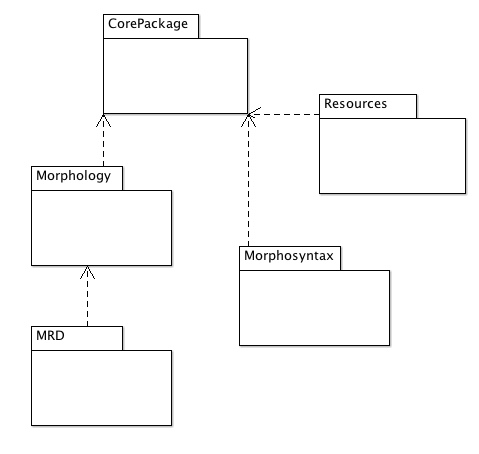
\includegraphics[scale=0.9]{../uml/export/ClassDiagramLMF.png}}}
\caption{LMF packages}
\end{figure}

\pagebreak % Core Package
Le \textit{core package} est divis\'e en deux sous-syst\`emes~:
\begin{itemize}
\item l'entr\'ee lexicale et ses diff\'erentes formes (signifiant) ;
\item le ou les sens (signifi\'e).
\end{itemize}

\begin{figure}[h]
\centerline{\fbox{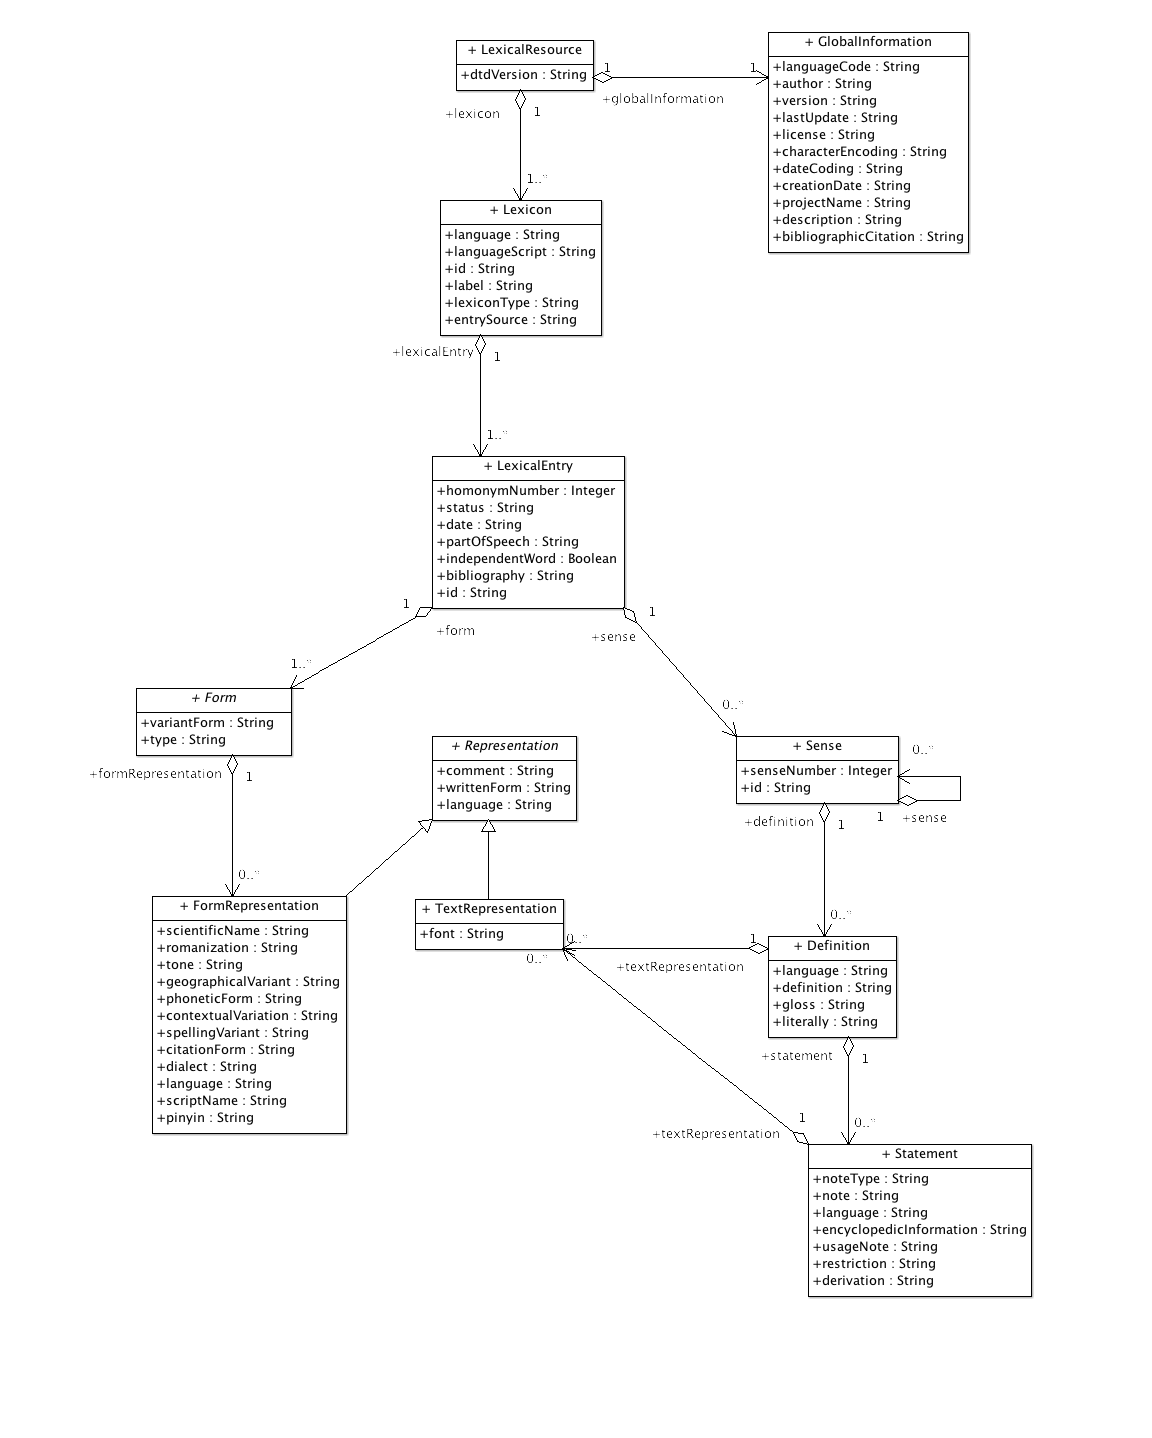
\includegraphics[width=12cm]{../uml/export/ClassDiagramCorePackage.png}}}
\caption{Core Package}
\end{figure}

\pagebreak % existing extensions

Les syst\`emes p\'eriph\'eriques (extensions) sont souples, optionnels, mais puissants. Parmi les 8 extensions propos\'ees, j'en ai s\'electionn\'ees certaines qui me paraissaient pertinentes pour nos besoins.

\begin{figure}[h]
\centerline{\fbox{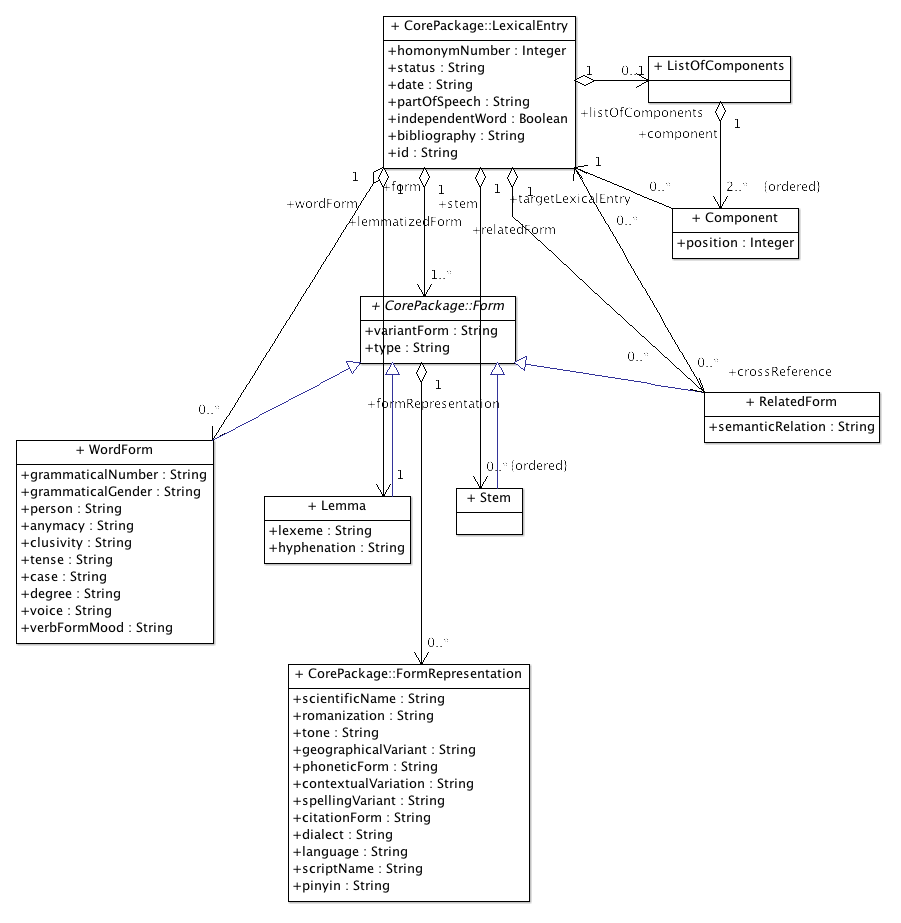
\includegraphics[width=15cm]{../uml/export/ClassDiagramMorphology.png}}}
\caption{Morphology}
\end{figure}
\pagebreak
\begin{figure}[htp]
\centerline{\fbox{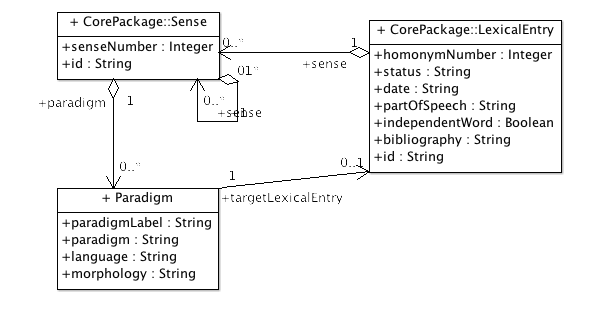
\includegraphics[width=12cm]{../uml/export/ClassDiagramMorphosyntax.png}}}
\caption{Morphosyntax}
\end{figure}
\nopagebreak
\begin{figure}[h]
\centerline{\fbox{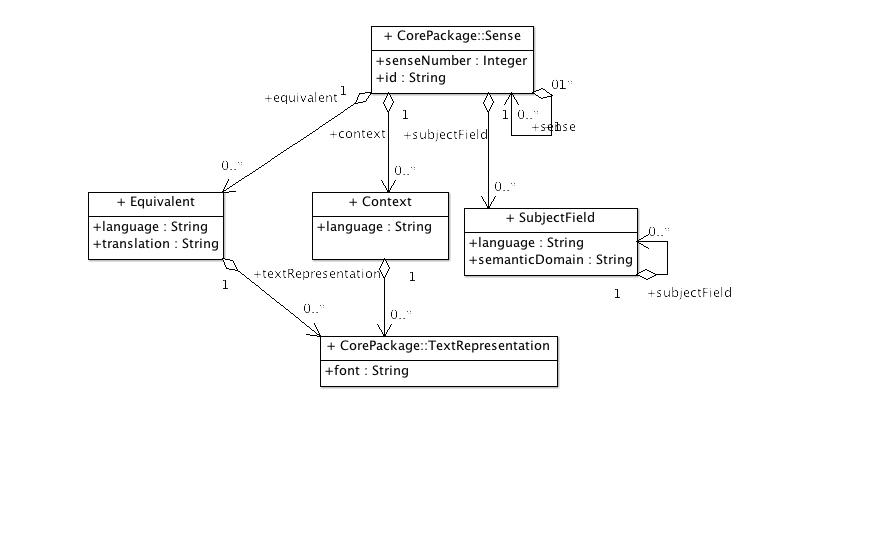
\includegraphics[width=14cm]{../uml/export/ClassDiagramMRD.png}}}
\caption{MRD}
\end{figure}

\pagebreak % created extensions

En plus des extensions existantes, on peut en cr\'eer. C'est ce que je propose de faire pour la gestion des ressources audio et des locuteurs.

\begin{figure}[h]
\centerline{\fbox{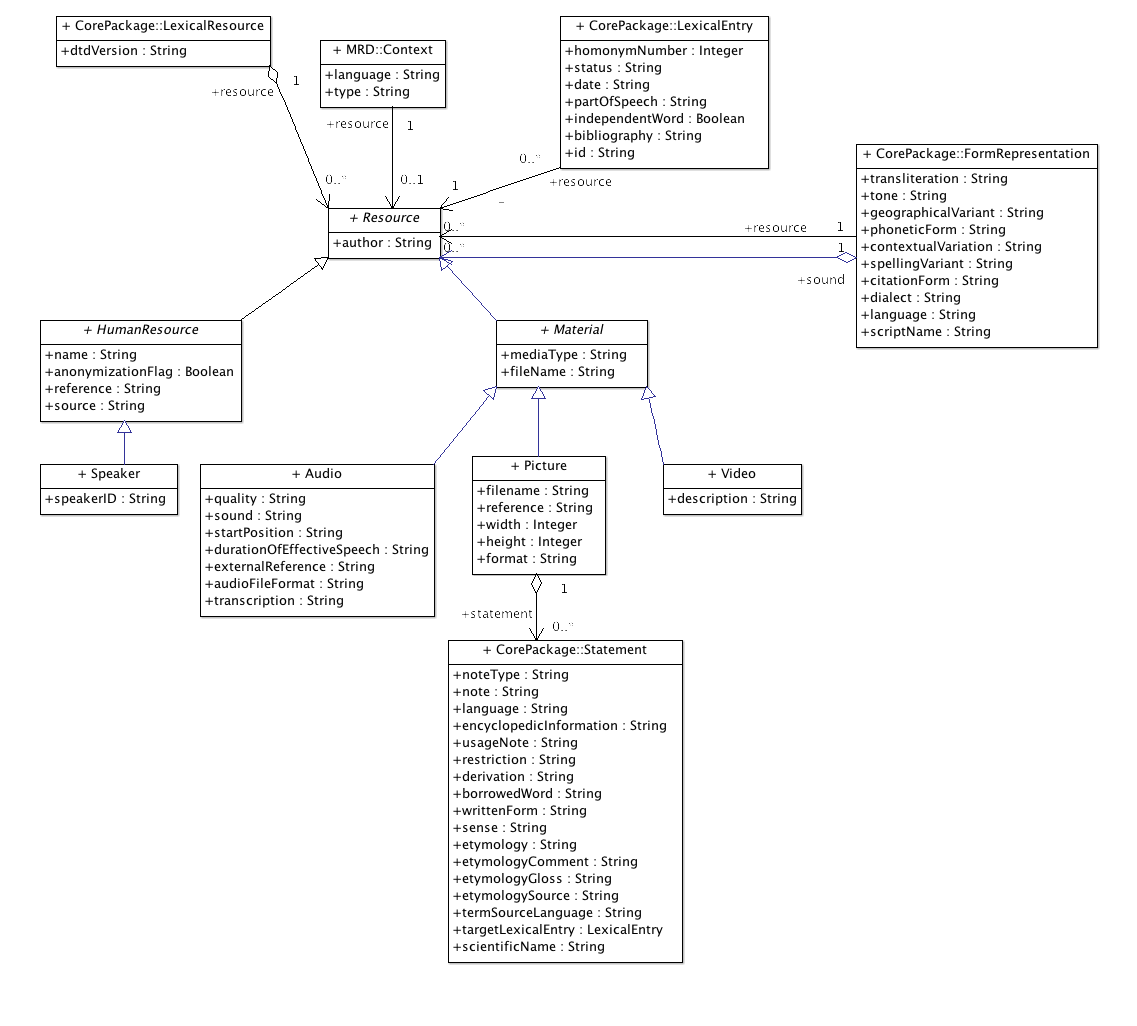
\includegraphics[width=15cm]{../uml/export/ClassDiagramResources.png}}}
\caption{Resources}
\end{figure}

\newpage
\section{Classes et attributs}

Dans cette section, je vais m'attarder sur ce que sont une classe et ses attributs - de mani\`ere simplifi\'ee rassurez-vous. Pourquoi~? Car il y a en fait une correspondance directe entre l'architecture logicielle utilis\'ee et le format XML LMF choisi.

\subsection{Correspondance entre UML et XML}

Un petit exemple afin de visualiser : prenons la classe \textit{Statement} du \textit{Core Package} (en bas \`a droite de la figure). Cette classe comporte de nombreux attributs, dont les 2 suivants :
\begin{itemize}
\item \textit{borrowed word}
\item \textit{written form}
\end{itemize}
En suivant les recommandations LMF, si l'on souhaite par exemple repr\'esenter un emprunt de l'anglais du mot \textit{cool}, on obtient les lignes XML suivantes :
\begin{lstlisting}
<Statement>
	<feat att=''borrowed word'' val=''eng''/>
	<feat att=''written form'' val='cool''/>
</Statement>
\end{lstlisting}
Plusieurs commentaires sur cet exemple :
\begin{itemize}
\item En LMF, les attributs de classe sont strutur\'es en tant que paire d'attributs de la balise sp\'ecifique \textit{feat}.
\begin{itemize}
\item Le nom de l'attribut est en fait la valeur de l'attribut \textit{att} de la balise \textit{feat} ;
\item La valeur donn\'ee \`a cet attribut est la valeur de l'attribut \textit{val} de la balise \textit{feat}.
\end{itemize}
\item Dans cet exemple, il est \`a noter que conform\'emement \`a LMF (et d'ailleurs aussi MDF), la langue d'emprunt doit \^etre renseign\'ee dans l'attribut \textit{borrowed word}, tandis que le mot d'emprunt, lui, est renseign\'e dans l'attribut \textit{written form}.
\end{itemize}

\section{Pour les novices : qu'est-ce qu'une classe ?}

Une classe est une entit\'e abstraite qui repr\'esente un objet, par exemple une voiture, et qui comporte certains attributs, par exemple la marque ou la couleur de la voiture. Une classe a \'egalement ce qu'on appelle des m\'ethodes, c'est-\`a-dire des fonctions qu'elle impl\'emente : pour une voiture, ce serait par exemple d\'emarrer, acc\'el\'erer, etc. Alors que les attributs sont en r\`egle g\'en\'erale mat\'erialis\'es par des noms communs, les m\'ethodes, elles, sont nomm\'ees par des verbes d'action.\\
D'autre part, une classe peut d\'eriver d'une autre classe, c'est-\`a-dire en simplifiant qu'elle h\'erite des attributs et des m\'ethodes de sa classe m\`ere. Cet h\'eritage est repr\'esent\'e sur les sch\'emas UML qui pr\'ec\`edent par une fl\`eche pleine. Par exemple, on pourrait imaginer une classe v\'ehicule, de laquelle d\'eriveraient les classes voiture, moto, etc. Ils auraient tous des attributs en commun (nombre de roues, de portes, marque, couleur du v\'ehicule, etc.) qui seraient donc des attributs de la classe v\'ehicule, et des attributs sp\'ecifiques comme par exemple la b\'equille pour une moto ou un v\'elo.\\
Une classe peut avoir une relation d'agr\'egation ou de composition avec une autre classe, c'est-\`a-dire qu'elle en fait partie. Si l'on reprend l'exemple classique de la voiture, et si l'on cr\'ee une classe roue, on pourrait dire que la voiture est compos\'ee, entre autres, de 4 roues. Cette relation est sch\'ematis\'ee par un losange en UML.\\
Une dernière relation utilis\'ee dans les sch\'emas UML de la section pr\'ec\'edente est une simple fl\`eche, qui signifie qu'une classe en r\'ef\'erence une autre. Par exemple, une voiture et son propri\'etaire sont deux entit\'es bien distinctes qui existent ind\'ependamment l'une de l'autre. Cependant, il existe bien un lien entre ces deux entit\'es, repr\'esent\'e par une association.\\
Enfin, en UML, les classes abstraites sont not\'ees en italique.

\subsection{Classes et attributs d\'efinis par LMF}

Pour chacun des \textit{packages} d\'ecrits dans la section pr\'ec\'edente, des classes et des relations entre ces classes sont d\'efinies et non modifiables (\`a noter que certains projets existants d\'evient un peu du standard en proposant des am\'eliorations). Par contre, nous sommes (plus ou moins) libres de d\'efinir les attributs que nous souhaitons pour chacune de ces classes. Cependant, chaque attribut doit \^etre r\'ef\'erenc\'e dans le DCR (\textit{Data Category Registry}). On peut utiliser les \'el\'ements existants, ou bien en proposer de nouveaux le cas \'ech\'eant. Il s'agit d'une base de donn\'ees ouverte, accessible sur le site \url{http://www.isocat.org}.\\
Une difficult\'e que j'ai rencontr\'ee avec cette base de donn\'ees, c'est qu'il y a beaucoup de redondance, de doublons : beaucoup de termes quasi-identiques sont d\'efinis 2 ou 3 fois. Dans ces cas-l\`a, lequel choisir ? Sur quels crit\`eres ? J'ai tent\'e de privil\'egier la d\'efinition qui se rapprochait le plus du besoin, et \`a d\'efinition \`a peu pr\`es similaire, j'ai privil\'egi\'e les termes issus de MDF, ou cr\'e\'es par Gil Francopoulo (l'auteur du livre sur LMF). Cependant, plut\^ot que suivre le principe de MDF concernant les marqueurs associ\'es sp\'ecifiquement aux langages vernaculaire, r\'egional et national, j'ai choisi de laisser davantage de libert\'e en définissant un attribut g\'en\'eral associ\'e \`a un attribut de langue (exemple : d\'efinition dans la langue 'xxx' plut\^ot que 'dn' qui impose une d\'efinition dans une langue nationale pr\'ed\'efinie). Ce qui en outre \'evite d'avoir \`a d\'efinir 'df' par exemple pour le fran\c{c}ais.\\

Dans le tableau ci-dessous, je n'ai list\'e que les attributs de chaque classe, et non les m\'ethodes, car cela alourdirait les sp\'ecifications sans apporter d'informations pertinentes. J'ai \'egalement noter les marqueurs MDF auxquels les attributs font r\'ef\'erence s'ils existent. Quant \`a l'extension LMF concern\'ee, elle se trouve dans la colonne \textit{LMF package}.

\pagebreak

\begin{center}
\begin{longtable}{*7{p{2cm}}}
\caption[]{LMF classes and their attributes} \\ \hline\hline
\textbf{LMF package} & \textbf{Class name} & \textbf{Attribute} & \textbf{Attribute type or example value} & \textbf{DCR PID and type} & \textbf{MDF marker} & \textbf{Comment} \\ \hline\hline
\endfirsthead
\caption[]{(continued)} \\
\textbf{LMF package} & \textbf{Class name} & \textbf{Attribute} & \textbf{Attribute type or example value} & \textbf{DCR PID and type} & \textbf{MDF marker} & \textbf{Comment} \\
\endhead
\endfoot
\endlastfoot
% CORE PACKAGE
% Lexical Resource
\multirow{82}{2cm}{Core Package} & \multirow{4}{2cm}{Lexical Resource (singleton)} & dtd version & ``16'' & - & - & LMF DTD is an XML attribute \\ \cmidrule{3-7}
& & global information & Global Information & N/A & N/A & \\ \cmidrule{3-7}
& & lexicon & Lexicon & N/A & N/A & \\ \cmidrule{3-7}
& & resource & Speaker & N/A & N/A & \\ \cmidrule{2-7}
% Global Information
& \multirow{11}{2cm}{Global Information (no subclass)} & language code & ``ISO-639-3'' & \href{http://www.isocat.org/datcat/DC-2008}{2008} open & - & \\ \cmidrule{3-7}
& & date coding & ``ISO-8601” & \href{http://www.isocat.org/datcat/DC-2090}{2090} open & - & \\ \cmidrule{3-7}
& & creation date & ``2001-03-24” & \href{http://www.isocat.org/datcat/DC-2510}{2510} open & - & \\ \cmidrule{3-7}
& & last update & ``2014-07-21” & \href{http://www.isocat.org/datcat/DC-2526}{2526} open & - & \\ \cmidrule{3-7}
& & author & ``Alexis Michaud, MICA \& Guillaume Jacques, CRLAO” & \href{http://www.isocat.org/datcat/DC-6130}{6130} open & - & \\ \cmidrule{3-7}
& & version & ``0.1” & \href{http://www.isocat.org/datcat/DC-2547}{2547} open & - & \\ \cmidrule{3-7}
& & license & ``GPL” & \href{http://www.isocat.org/datcat/DC-2457}{2457} open & - & \\ \cmidrule{3-7}
& & project name & ``ANR HimalCo” & \href{http://www.isocat.org/datcat/DC-2536}{2536} open & - & \\ \cmidrule{3-7}
& & description & ``everything you want to tell about this resource” & \href{http://www.isocat.org/datcat/DC-2520}{2520} open & - & \\ \cmidrule{3-7}
& & bibliographic citation & ``Online dictionaries, CNRS, 2014” & \href{http://www.isocat.org/datcat/DC-6137}{6137} open & - & \\ \cmidrule{3-7}
& & character encoding & ``UTF-8” & \href{http://www.isocat.org/datcat/DC-2564}{2564} open & - & \\ \cmidrule{3-7}
% Lexicon
& \multirow{7}{2cm}{Lexicon (no subclass)} & id & ``na?'' & \href{http://www.isocat.org/datcat/DC-1845}{1845} open & - & identifier is an XML attribute \\ \cmidrule{3-7}
& & label & ``Na online dictionary'' & \href{http://www.isocat.org/datcat/DC-1857}{1857} open & - & \\ \cmidrule{3-7}
& & language & ``fra'', ``eng'' & \href{http://www.isocat.org/datcat/DC-2482}{2482} constrained & - & ISO 639 ; vernacular language \\ \cmidrule{3-7}
& & language script & ``latn'' & \href{http://www.isocat.org/datcat/DC-2485}{2485} open & - & ISO 15924 \\ \cmidrule{3-7}
& & lexicon type & ``bilingual dictionary na - eng'' & \href{http://www.isocat.org/datcat/DC-2487}{2487} open & - & \\ \cmidrule{3-7}
& & entry source & ``na\_dic\-tio\-na\-ry.txt'' & \href{http://www.isocat.org/datcat/DC-207}{207} open & - & \\ \cmidrule{3-7}
& & vowel harmony & & no existing DC & - & \\ \cmidrule{3-7}
& & lexical entry & Lexical Entry & N/A & N/A & - \\ \cmidrule{2-7}
% Lexical Entry
& \multirow{16}{2cm}{Lexical Entry (no subclass)} & id & ``toto\_1'' & \href{http://www.isocat.org/datcat/DC-6196}{6196} open & lx \textless id\textgreater, se \textless id\textgreater & unique identifier or key form is an XML attribute \\ \cmidrule{3-7}
& & part of speech (English) & ``verb'' & \href{http://www.isocat.org/datcat/DC-3748}{3748} closed \hyperlink{1}{(1)} \hypertarget{pos}{} & ps & grammatical category \\ \cmidrule{3-7}
& & lemmatized form & Lemma & N/A & N/A & \\ \cmidrule{3-7}
& & date & ``2014-06-15'' & \href{http://www.isocat.org/datcat/DC-3694}{3694} open & dt & \\ \cmidrule{3-7}
& & status & ``no print'', ``done'', ``check'' & \href{http://www.isocat.org/datcat/DC-3760}{3760} open & st & \\ \cmidrule{3-7}
& & homonym number & ``1'' & \href{http://www.isocat.org/datcat/DC-3714}{3714} open & hm & ``0'' if no homonym \\ \cmidrule{3-7}
& & bibliography & ``212'' & \href{http://www.isocat.org/datcat/DC-3687}{3687} open & bb & \\ \cmidrule{3-7}
& & independent word & yes, no & \href{http://www.isocat.org/datcat/DC-5285}{5285} closed & & \\ \cmidrule{3-7}
& & resource & Audio & N/A & N/A & \\ \cmidrule{3-7}
& & form & Form Re\-pre\-sen\-ta\-tion & N/A & N/A & \\ \cmidrule{3-7}
& & sense & Sense & N/A & N/A & \\ \cmidrule{3-7}
& & word form & Word Form & N/A & N/A & \\ \cmidrule{3-7}
& & related form & Related Form & N/A & N/A & \\ \cmidrule{3-7}
& & stem & Stem & N/A & N/A & \\ \cmidrule{3-7}
& & list of components & List Of Components & N/A & N/A & \\ \cmidrule{3-7}
& & borrowed word & Borrowed Word & N/A & N/A & \\ \cmidrule{2-7}
% Form
& \multirow{3}{2cm}{Form (abstract class)} & variant form(s) & ``woman'', ``women'' & \href{http://www.isocat.org/datcat/DC-3768}{3768} open & va, pdl \textless stem\textgreater & written or spoken \\ \cmidrule{3-7}
& & type & \hyperlink{2}{(2)} \hypertarget{type}{} & \href{http://www.isocat.org/datcat/DC-1971}{1971} open & & variant type : spelling, pronunciation, archaic, etc. \\ \cmidrule{3-7}
& & form representation & Form Re\-pre\-sen\-ta\-tion & N/A & N/A & \\ \cmidrule{2-7}
% Form Representation
& \multirow{14}{2cm}{Form Re\-pre\-sen\-ta\-tion} & tone & & \href{http://www.isocat.org/datcat/DC-517}{517} open & np \textless tone\textgreater & \\ \cmidrule{3-7}
& & geographical variant & & \href{http://www.isocat.org/datcat/DC-1851}{1851} open & va & \\ \cmidrule{3-7}
& & phonetic form (vernacular) & & \href{http://www.isocat.org/datcat/DC-3745}{3745} open & ph & \\ \cmidrule{3-7}
& & contextual variation & & \href{http://www.isocat.org/datcat/DC-1977}{1977} open & lc & \\ \cmidrule{3-7}
& & spelling variant & & \href{http://www.isocat.org/datcat/DC-5612}{5612} open & a & \\ \cmidrule{3-7}
& & citation form (vernacular) & & \href{http://www.isocat.org/datcat/DC-3716}{3716} open & lc & \\ \cmidrule{3-7}
& & dialect & ``North German'' & \href{http://www.isocat.org/datcat/DC-2466}{2466} open & ve & \\ \cmidrule{3-7}
& & language & ``fra'', ``eng'' & \href{http://www.isocat.org/datcat/DC-2482}{2482} constrained & - & ISO 639 ; language used for variant comment \\ \cmidrule{3-7}
& & trans\-li\-te\-ra\-tion & ``readable characters'' & \href{http://www.isocat.org/datcat/DC-1848}{1848} open & ph & \\ \cmidrule{3-7}
& & script name & ``Latin'' & \href{http://www.isocat.org/datcat/DC-3809}{3809} open & - & script used for romanization \\ \cmidrule{3-7}
& & resource & Speaker & N/A & N/A & \\ \cmidrule{3-7}
& & sound & Audio & N/A & N/A & \\ \cmidrule{2-7}
% Representation
& \multirow{3}{2cm}{Re\-pre\-sen\-ta\-tion (abstract class)} & written form & ``...'' & \href{http://www.isocat.org/datcat/DC-1836}{1836} open & xv, xe, xn, xr, xf & example \\ \cmidrule{3-7}
& & language & ``fra'', ``eng'' & \href{http://www.isocat.org/datcat/DC-2482}{2482} constrained & - & ISO 639 ; language used for variant comment \\ \cmidrule{3-7}
& & comment & ``...'' & \href{http://www.isocat.org/datcat/DC-1846}{1846} open & ve, vn, vr, vf, xc & explanation \\ \cmidrule{2-7}
% Text Representation
& \multirow{1}{2cm}{Text Re\-pre\-sen\-ta\-tion} & font & font family / font weight / font size & \href{http://www.isocat.org/datcat/DC-1650}{1650} closed & & 'font-style', 'font-variant', 'line-height' \\ \cmidrule{2-7}
% Sense
& \multirow{9}{2cm}{Sense} & id & ``toto\_1\_1'' & \href{http://www.isocat.org/datcat/DC-1845}{1845} open & - & identifier or key form is an XML attribute \\ \cmidrule{3-7}
& & sense number & ``1'' & \href{http://www.isocat.org/datcat/DC-3758}{3758} open & sn & \\ \cmidrule{3-7}
& & sense & Sense & N/A & N/A & \\ \cmidrule{3-7}
& & definition & Definition & N/A & N/A & \\ \cmidrule{3-7}
& & etymology & Etymology & N/A & N/A & \\ \cmidrule{3-7}
& & paradigm & Paradigm & N/A & N/A & \\ \cmidrule{3-7}
& & equivalent & Equivalent & N/A & N/A & \\ \cmidrule{3-7}
& & context & Context & N/A & N/A & \\ \cmidrule{3-7}
& & subject field & Subject Field & N/A & N/A & \\ \cmidrule{2-7}
% Definition
& \multirow{6}{2cm}{Definition} & definition & ``This is the lexeme definition'' & \href{http://www.isocat.org/datcat/DC-1972}{1972} open & dv, de, dn, dr, df & \\ \cmidrule{3-7}
& & gloss & ``\scshape{GLOSS}'' & \href{http://www.isocat.org/datcat/DC-244}{244} open & gv, ge, gn, gr, gf & \\ \cmidrule{3-7}
& & language & ``fra'', ``eng'' & \href{http://www.isocat.org/datcat/DC-2482}{2482} constrained & - & ISO 639 ; language used for definition and gloss \\ \cmidrule{3-7}
& & literally & 'au pied de la lettre' & \href{http://www.isocat.org/datcat/DC-3721}{3721} open & lt & \\ \cmidrule{3-7}
& & text representation & Text Re\-pre\-sen\-ta\-tion & N/A & N/A & \\ \cmidrule{3-7}
& & statement & Statement & N/A & N/A & \\ \cmidrule{2-7}
% Statement
& \multirow{8}{2cm}{Statement} & note type & \hyperlink{3}{(3)} \hypertarget{nt}{} & \href{http://www.isocat.org/datcat/DC-6178}{6178} open & nt \textless type\textgreater, np \textless type\textgreater, ng \textless type\textgreater & \\ \cmidrule{3-7}
& & note & & \href{http://www.isocat.org/datcat/DC-382}{382} open & na, nd, ng, np, nq, ns, nt & \\ \cmidrule{3-7}
& & language & ``fra'', ``eng'' & \href{http://www.isocat.org/datcat/DC-2482}{2482} constrained & nt \textless lang\textgreater & ISO 639 \\ \cmidrule{3-7}
& & encyclopedic information & ``...'' & \href{http://www.isocat.org/datcat/DC-3828}{3828} open & ee, en, er, ev & \\ \cmidrule{3-7}
& & usage note & ``...'' & \href{http://www.isocat.org/datcat/DC-526}{526} open & uv, ue, un, ur & text \\ \cmidrule{3-7}
& & restriction & ``...'' & \href{http://www.isocat.org/datcat/DC-1956}{1956} open & oe, on, or, ov & \\ \cmidrule{3-7}
& & derivation & ``...'' & \href{http://www.isocat.org/datcat/DC-188}{188} open & - & \\ \cmidrule{3-7}
& & borrowed word (English) & ``Chinese'' & \href{http://www.isocat.org/datcat/DC-3688}{3688} open & bw & source language \\ \cmidrule{3-7}
& & written form & ``...'' & \href{http://www.isocat.org/datcat/DC-1836}{1836} open & bw & loan word \\ \cmidrule{3-7}
& & sense & ``...'' & \href{http://www.isocat.org/datcat/DC-464}{464} open & - & sense in borrowed language \\ \cmidrule{3-7}
& & etymology & ``aspirin: from acetyl + spiraeic acid (old name for salicylic acid)'' & \href{http://www.isocat.org/datcat/DC-221}{221} open & et & \\ \cmidrule{3-7}
& & etymology comment (English) & & \href{http://www.isocat.org/datcat/DC-3696}{3696} open & ec & \\ \cmidrule{3-7}
& & target lexical entry & Lexical Entry & & cf \textless type=''et''\textgreater & \\ \cmidrule{3-7}
& & term source language & ``fra'', ``eng'' & \href{http://www.isocat.org/datcat/DC-3639}{3639} open & - & language \\ \cmidrule{3-7}
& & etymology gloss & & \href{http://www.isocat.org/datcat/DC-3698}{3698} open & eg & \\ \cmidrule{3-7}
& & etymology source & & \href{http://www.isocat.org/datcat/DC-3701}{3701} & es & \\ \cmidrule{3-7}
& & scientific name & ``Canis lupus familiaris'' & \href{http://www.isocat.org/datcat/DC-3754}{3754} open & sc & \\ \cmidrule{3-7}
& & text representation & Text Re\-pre\-sen\-ta\-tion & N/A & N/A & \\ \cmidrule{1-7}
% MORPHOLOGY
% List Of Components
\multirow{18}{2cm}{Morphology} &List Of Components & component & Component & N/A & N/A & \\ \cmidrule{2-7}
% Component
& \multirow{2}{2cm}{Component} & position & ``2'' & \href{http://www.isocat.org/datcat/DC-2183}{2183} open & - & \\ \cmidrule{3-7}
& & target lexical entry & Lexical Entry & N/A & N/A & \\ \cmidrule{2-7}
% Word Form
& \multirow{10}{2cm}{Word Form} & grammatical number & collective, dual, paucal, plural, quadrial, singular, trial & \href{http://www.isocat.org/datcat/DC-1298}{1298} closed & & \\ \cmidrule{3-7}
& & grammatical gender & common gender, feminine, masculine, neuter & \href{http://www.isocat.org/datcat/DC-1297}{1297} closed & & \\ \cmidrule{3-7}
& & person & first person, second person, third person & \href{http://www.isocat.org/datcat/DC-1328}{1328} closed & & \\ \cmidrule{3-7}
& & anymacy & animate, inanimate, other anymacy & \href{http://www.isocat.org/datcat/DC-1902}{1902} closed & & \\ \cmidrule{3-7}
& & clusivity & inclusive, exclusive & \href{http://www.isocat.org/datcat/DC-3031}{3031} closed & & \\ \cmidrule{3-7}
& & tense & future, imperfect, past, present & \href{http://www.isocat.org/datcat/DC-1286}{1286} closed & & \\ \cmidrule{3-7}
& & voice & active voice, middle voice, passive voice & \href{http://www.isocat.org/datcat/DC-1413}{1413} closed & & \\ \cmidrule{3-7}
& & verb form mood & \hyperlink{4}{(4)} \hypertarget{mood}{} & \href{http://www.isocat.org/datcat/DC-1427}{1427} closed & & \\ \cmidrule{3-7}
& & case & ``accusative case'' & \href{http://www.isocat.org/datcat/DC-1840}{1840} closed & & \\ \cmidrule{3-7}
& & degree & comparative degree, positive degree, superlative degree & \href{http://www.isocat.org/datcat/DC-2779}{2779} closed & & \\ \cmidrule{2-7}
% Lemma
& \multirow{2}{2cm}{Lemma} & lexeme & ``toto'' & \href{http://www.isocat.org/datcat/DC-3723}{3723} open & lx & \\ \cmidrule{3-7}
& & hyphenation & ``pho-ne-ti-cian'' & \href{http://www.isocat.org/datcat/DC-264}{264} open & - & syllables separated by '-' \\ \cmidrule{2-7}
% Stem
& \multirow{1}{2cm}{Stem} & & & N/A & N/A & \\ \cmidrule{2-7}
% Related Form
& \multirow{2}{2cm}{Related Form} & semantic relation & \hyperlink{5}{(5)} \hypertarget{relation}{} & \href{http://www.isocat.org/datcat/DC-6331}{6331} open & sy, an, cf \textless et\textgreater, cf \textless hm\textgreater, se, mn, lf, ev, ee, en, er & \\ \cmidrule{3-7}
& & cross reference & Lexical Entry & \href{http://www.isocat.org/datcat/DC-164}{164} open & cf, mn & also used for main entry cross-reference \\ \cmidrule{1-7}
% MORPHOSYNTAX
% Paradigm
\multirow{5}{2cm}{\textit{Mor\-pho\-syn\-tax}} & \multirow{5}{2cm}{Paradigm} & paradigm label (English) & \hyperlink{6}{(6)} \hypertarget{paradigm}{} & \href{http://www.isocat.org/datcat/DC-3741}{3741} open & pdl & \\ \cmidrule{3-7}
& & language & ``fra'', ``eng'' & \href{http://www.isocat.org/datcat/DC-2482}{2482} constrained & - & ISO 639 \\ \cmidrule{3-7}
& & paradigm & & \href{http://www.isocat.org/datcat/DC-3736}{3736} open & pd & \\ \cmidrule{3-7}
& & morphology (vernacular) & & \href{http://www.isocat.org/datcat/DC-3738}{3738} open & mr & \\ \cmidrule{3-7}
& & target lexical entry & Lexical Entry & N/A & N/A & in case of classifier \\ \cmidrule{1-7}
% MRD
% Context
\multirow{9}{2cm}{MRD} & \multirow{3}{2cm}{Context} & language & ``fra'', ``eng'' & \href{http://www.isocat.org/datcat/DC-2482}{2482} constrained & - & ISO 639 \\ \cmidrule{3-7}
& & type & ``proverb'', ``locution'', ``example'', ``combination'' & \href{http://www.isocat.org/datcat/DC-1971}{1971} open & PHONO & \\ \cmidrule{3-7}
& & resource & Audio & N/A & N/A & \\ \cmidrule{3-7}
& & text representation & Text Re\-pre\-sen\-ta\-tion & N/A & N/A & \\ \cmidrule{2-7}
% Subject Field
& \multirow{3}{2cm}{Subject Field} & language & ``fra'', ``eng'' & \href{http://www.isocat.org/datcat/DC-2482}{2482} constrained & sd \textless lang\textgreater & ISO 639 \\ \cmidrule{3-7}
& & semantic domain & ``arbre'' & \href{http://www.isocat.org/datcat/DC-3755}{3755} open & sd, is, th & see appendix C of the MDF guide \\ \cmidrule{3-7}
& & subject field & Subject Field & N/A & N/A & hyponym / hypernym \\ \cmidrule{2-7}
% Equivalent
& \multirow{3}{2cm}{Equivalent} & language & ``fra'', ``eng'' & \href{http://www.isocat.org/datcat/DC-2482}{2482} constrained & - & ISO 639 \\ \cmidrule{3-7}
& & translation & & \href{http://www.isocat.org/datcat/DC-6037}{6037} open & re, rn, rr, rf & reversal \\ \cmidrule{3-7}
& & text representation & Text Re\-pre\-sen\-ta\-tion & N/A & N/A & \\ \cmidrule{1-7}
% RESOURCES
% Resource
\multirow{19}{2cm}{\textit{Resources}} & \multirow{1}{2cm}{Resource (abstract class)} & author & ``Guillaume Jacques, CRLAO'' & \href{http://www.isocat.org/datcat/DC-6130}{6130} open & - & \\ \cmidrule{2-7}
% Material
& \multirow{2}{2cm}{Material (abstract class)} & media type & unspecified, unknown, audio, video, document, text, image, drawing & \href{http://www.isocat.org/datcat/DC-2570}{2570} closed & & \\ \cmidrule{3-7}
& & file name & & \href{http://www.isocat.org/datcat/DC-5435}{5435} open & sf, sfx & \\ \cmidrule{2-7}
% Audio
& \multirow{7}{2cm}{Audio} & quality & very low, low, normal, good, very good (high) & \href{http://www.isocat.org/datcat/DC-2574}{2574} & sf, sfx \textless quality\textgreater & \\ \cmidrule{3-7}
& & sound & & \href{http://www.isocat.org/datcat/DC-2250}{2250} open & - & \\ \cmidrule{3-7}
& & transcription & & \href{http://www.isocat.org/datcat/DC-1849}{1849} open & - & \\ \cmidrule{3-7}
& & start position & ``00:05:00'' & \href{http://www.isocat.org/datcat/DC-3896}{3896} open & - & \\ \cmidrule{3-7}
& & duration of effective speech & ``00:05:00'', ``3'' & \href{http://www.isocat.org/datcat/DC-2691}{2691} open & - & \\ \cmidrule{3-7}
& & external reference & & \href{http://www.isocat.org/datcat/DC-1975}{1975} open & sf, sfx \textless numbering\textgreater & \\ \cmidrule{3-7}
& & audio file format & ``MP3'', ``Vorbis'', ``WAV'', ``AU'', ``uLaw'' & \href{http://www.isocat.org/datcat/DC-2689}{2689} open & sf, sfx & \\ \cmidrule{2-7}
% Video
& \multirow{1}{2cm}{Video} & description & ``everything you want to tell about this video'' & \href{http://www.isocat.org/datcat/DC-2520}{2520} open & - & \\ \cmidrule{2-7}
% Picture
& \multirow{3}{2cm}{Picture} & size & & \href{http://www.isocat.org/datcat/DC-2580}{2580}open & pc & \\ \cmidrule{3-7}
& & size unit & & \href{http://www.isocat.org/datcat/DC-2583}{2583} open & pc & \\ \cmidrule{3-7}
& & statement & Statement & & N/A & \\ \cmidrule{2-7}
% Human Resource
& \multirow{4}{2cm}{Human Resource (abstract class)} & name & & \href{http://www.isocat.org/datcat/DC-6122}{6122} open & - & \\ \cmidrule{3-7}
& & source & & \href{http://www.isocat.org/datcat/DC-3759}{3759} open & so & \\ \cmidrule{3-7}
& & reference & & \href{http://www.isocat.org/datcat/DC-3751}{3751} open & rf & \\ \cmidrule{3-7}
& & a\-no\-ny\-mi\-za\-tion flag & false, true, unknown, unspecified & \href{http://www.isocat.org/datcat/DC-2548}{2548} closed & so \textless print\textgreater & \\ \cmidrule{2-7}
% Speaker
& \multirow{1}{2cm}{Speaker} & speaker id & ``SpID-1'' & \href{http://www.isocat.org/datcat/DC-3597}{3597} open & & \\ \hline\hline
\end{longtable}
\end{center}

\hypertarget{1}{(1)}
\hyperlink{pos}{part of speech:}
\begin{itemize}
\item adjective \href{http://www.isocat.org/datcat/DC-1230}{1230}
\item adposition \href{http://www.isocat.org/datcat/DC-1231}{1231}
\item adverb \href{http://www.isocat.org/datcat/DC-1232}{1232}
\item conjunction \href{http://www.isocat.org/datcat/DC-1260}{1260}
\item determiner \href{http://www.isocat.org/datcat/DC-1272}{1272}
\item interjection \href{http://www.isocat.org/datcat/DC-1318}{1318}
\item noun \href{http://www.isocat.org/datcat/DC-1333}{1333}
\item numeral \href{http://www.isocat.org/datcat/DC-1334}{1334}
\item particle \href{http://www.isocat.org/datcat/DC-3372}{3372}
\item pronoun \href{http://www.isocat.org/datcat/DC-1370}{1370}
\item verb \href{http://www.isocat.org/datcat/DC-1424}{1424}
\item ideophone \href{http://www.isocat.org/datcat/DC-4192}{4192}
\item transitive verb \href{http://www.isocat.org/datcat/DC-1405}{1405}
\item intransitive verb \href{http://www.isocat.org/datcat/DC-1322}{1322}
\item reflexive verb \href{http://www.isocat.org/datcat/DC-5592}{5592}
\item negation \href{http://www.isocat.org/datcat/DC-2313}{2313}
\item impersonal verb \href{http://www.isocat.org/datcat/DC-1306}{1306}
\item classifier \href{http://www.isocat.org/datcat/DC-2345}{2345}
\item preposition \href{http://www.isocat.org/datcat/DC-1366}{1366}
\item  bitransistive verb \href{http://www.isocat.org/datcat/DC-1275}{1275}
\item affix \href{http://www.isocat.org/datcat/DC-1234}{1234}
\item possessive pronouns \href{http://www.isocat.org/datcat/DC-1359}{1359}
\item particle
\end{itemize}
Valeurs non trouv\'ees dans la DCS (\textit{Data Category Selection}) :
\begin{itemize}
\item onomatope
\item function word
\item stative intransitive verb
\item linker
\end{itemize}

\hypertarget{2}{(2)}
\hyperlink{type}{type:}
\begin{itemize}
\item unspecified \href{http://www.isocat.org/datcat/DC-1908}{1908} (simple)
\item orthography \href{http://www.isocat.org/datcat/DC-2971}{2971} (simple)
\item phonetics \href{http://www.isocat.org/datcat/DC-2641}{2641} (simple)
\item archaic form \href{http://www.isocat.org/datcat/DC-504}{504} (simple)
\end{itemize}

\hypertarget{3}{(3)}
\hyperlink{nt}{note type:}
\begin{itemize}
\item ``comparison''
\item ``history''
\item ``semantics''
\item ``tone''
\item ``derivation''
\item ``case''
\item ``subord''
\item ``usage''
\item ``comment''
\item ``legend''
\item ``restriction''
\item ``encyclopedic''
\item ``anthropology''
\item ``discourse''
\item ``grammar''
\item ``phonology''
\item ``question''
\item ``sociolinguistics''
\item ``general''
\end{itemize}

\hypertarget{4}{(4)}
\hyperlink{mood}{verb form mood:}
\begin{itemize}
\item gerundive
\item imperative
\item indicative
\item infinitive
\item participle
\item subjunctive
\item conditional
\item relative mood
\item prohibitive mood
\item debitive mood
\end{itemize}

\hypertarget{5}{(5)}
\hyperlink{relation}{semantic relation:}
\begin{itemize}
\item synonym
\item antonym
\item homonym
\item etymology
\item subentry
\item main entry
\item simple link
\item derived form
\item root
\item stem
\item collocation \href{http://www.isocat.org/datcat/DC-340}{340} (simple) (classifier)
\end{itemize}

\hypertarget{6}{(6)}
\hyperlink{paradigm}{paradigm label:}
\begin{itemize}
\item lexicalized affix (la)
\item conjugation class (cc)
\item th\`eme du pass\'e (past)
\item comitatif (comit)
\item construction (constr)
\item directional (dir)
\item irregularity (ir)
\end{itemize}

\subsection{Remarques et limitations}

\begin{enumerate}
\item Les sous-entr\'ees de Toolbox sont cod\'ees comme des \textit{Lexical Entry} dont la principale a des liens vers les autres.
\item Avec le mod\`ele propos\'e, on ne peut pas mettre de r\'ef\'erence (`cf') d'un sens vers un autre sens. C'est au niveau de l'entr\'ee lexicale que l'on peut r\'ef\'erencer une autre entr\'ee lexicale en tant que synonyme par exemple. Est-ce qu'il y a un besoin de faire ça au niveau des 'sn' (\textit{sense number}) ? Cela ajoute de la complexit\'e au niveau du mod\`ele, mais c'est une am\'elioration possible. On peut aussi simplifier le mod\`ele si vous pensez que certains attributs voire certaines classes ne sont pas n\'ecessaires.
\item Cas des pr\'edicats complexes VV ou NV : prenons le cas du pr\'edicat complexe NV. En suivant ce mod\`ele LMF, on aurait 3 entr\'ees lexicales :
\begin{itemize}
\item V avec l'attribut \textit{independent word = no} ;
\item N avec l'attribut \textit{independent word = no} ;
\item NV avec l'attribut \textit{independent word = yes}, ayant comme liste de composants (\textit{List Of Components}) un lien vers les 2 entr\'ees lexicales d\'efinies ci-dessus.
\end{itemize}
\end{enumerate}

\pagebreak

\section{Exemples}

\subsection{Na}

\begin{center}
\begin{longtable}{|p{4cm}|p{11cm}|}
\caption[]{Na dictionary: matching between MDF and LMF} \\ \hline
\endfirsthead
\caption[]{(continued)} \\
\endhead
\endfoot
\endlastfoot
\textbf{MDF} & \textbf{LMF} \\ \hline
lx, se & Lemma lexeme \\ \hline
lx, se \textless id\textgreater & Lexical Entry id \\ \hline
sf & Material file name \\ \hline
sf \textless nb\textgreater & Audio external reference \\ \hline
hm & Lexical Entry homonym number \\ \hline
lc & Form Representation contextual variation \\ \hline
ph & Form Representation romanization \\ \hline
bw & Borrowed Word borrowed word / written form \\ \hline
et & Etymology etymology \\ \hline
ec & Etymology etymology comment \\ \hline
ec \textless lang\textgreater & Etymology language \\ \hline
ps & Lexical Entry part of speech \\ \hline
sn & Sense sense number \\ \hline
cf & Related Form cross reference \\ \hline
cf \textless type\textgreater & Related Form semantic relation \\ \hline
sd & Subject Field semantic domain \\ \hline
sd \textless lang\textgreater & Subject Field language \\ \hline
nt & Statement note \\ \hline
nt \textless lang\textgreater & Statement language \\ \hline
nt \textless type\textgreater & Statement note type \\ \hline
np & Statement note \\ \hline
np \textless type\textgreater & Statement note type \\ \hline
nd & Statement note \\ \hline
nd \textless arch\textgreater, ue archaic & Form type = archaic form \\ \hline
so & Human Resource source \\ \hline
so \textless print\textgreater & Human Resource anonymization flag \\ \hline
va & Form Representation variant form \\ \hline
va \textless speaker\textgreater & Form Representation resource \\ \hline
vf & Representation comment with Representation language = ``fra''  \\ \hline
vf \textless type\textgreater & Representation comment \\ \hline
pdl & Paradigm paradigm label \\ \hline
pdv & Paradigm paradigm with Paradigm language = ``na'' \\ \hline
pdf & Paradigm paradigm with Paradigm language = ``fra'' \\ \hline
de & Definition definition with Definition language = ``eng'' \\ \hline
ge & Definition gloss with Definition language = ``eng'' \\ \hline
dn & Definition definition with Definition language = ``chn'' \\ \hline
gn & Definition gloss with Definition language = ``chn'' \\ \hline
gr & Definition gloss with Definition language = ``...'' \\ \hline
df & Definition definition with Definition language = ``fra'' \\ \hline
gf & Definition gloss with Definition language = ``fra'' \\ \hline
xv & Representation written form with Representation language = ``na?'' \\ \hline
xe & Representation written form with Representation language = ``eng'' \\ \hline
xn & Representation written form with Representation language = ``chn'' \\ \hline
xf & Representation written form with Representation language = ``fra'' \\ \hline
rf & Context resource \\ \hline
xc & Representation comment \\ \hline
dt & Lexical Entry date \\ \hline
\end{longtable}
\end{center}

\pagebreak

\begin{quote}
\textbackslash lx \ipa{æ˩˧} \\
\textbackslash sf \textless nb="B"\textgreater~1789 \\
\textbackslash sf \textless nb="2011"\textgreater~2642 \\
\textbackslash hm \\
\textbackslash ph \\
\textbackslash bw \\
\textbackslash et \\
\textbackslash ec \textless lang="fr"\textgreater \\
\textbackslash ps n \\
\textbackslash sn \\
\textbackslash cf \\
\textbackslash cf \textless type="hm"\textgreater \\ 
\textbackslash sd \textless lang="fr"\textgreater~animal \\
\textbackslash sd \textless lang="eng"\textgreater~animal \\
\textbackslash nt \textless lang="pumi" type="comp" print="n"\textgreater \\
\textbackslash nt \textless type="hist" print="n"\textgreater \\
\textbackslash nt \textless type="hist" print="n"\textgreater \\
\textbackslash nt \textless type="sem"\textgreater \\
\textbackslash np LM confirmé type "porc" \\
\textbackslash np \textless type="tone"\textgreater~LM \\
\textbackslash nd \\
\textbackslash so \textless print="n"\textgreater~F4 \\
\textbackslash va \textless speaker="F4"\textgreater \\
\textbackslash vf \textless type="tone"\textgreater \\
\textbackslash va \textless speaker="F5"\textgreater~ID. \\
\textbackslash vf \textless type="tone"\textgreater \\
\textbackslash va \textless speaker="M18"\textgreater \\
\textbackslash va \textless speaker="M21"\textgreater~ID. \\
\textbackslash va \textless speaker="M23"\textgreater \\
\textbackslash pdl classifier \\
\textbackslash pdv \ipa{mi˩} \\
\textbackslash pdf \\
\textbackslash de chicken \\
\textbackslash ge chicken \\
\textbackslash dn \zh{鸡} \\
\textbackslash gn \zh{鸡} \\
\textbackslash gr \\
\textbackslash df poulet, poule \\
\textbackslash gf poulet \\
\textbackslash xv \ipa{æ˩ dzɯ˧-ze˩} \\
\textbackslash xe ...has eaten (a/some) chicken \\
\textbackslash xn \zh{吃了鸡} \\
\textbackslash begin{lstlisting} \\
\textbackslash xf ...a mangé (un/du) poulet \\
\textbackslash xc PHONO \\
\textbackslash xv \ipa{æ˩ hwæ˧-ze˧} \\
\textbackslash xe ...has bought (a) chicken \\
\textbackslash xn \zh{买了鸡} \\
\textbackslash xf ...a acheté (un/du) poulet \\
\textbackslash xc PHONO \\
\textbackslash xv \ipa{æ˩˥, | kʰv˧, | bo˩˥, | hwɤ˧˥, | ʝi˧, | lɑ˧, | tʰo˧li˧, | mv˧gv˧, | bv˧ʐv˧, | ʐwæ˧, | jo˧, | ʑi˩˥} \\
\textbackslash xe the twelve years of the duodenary cycle \\
\textbackslash xn \zh{十二个生肖} \\
\textbackslash xf les douze signes astrologiques \\
\textbackslash rf \\
\textbackslash xv \\
\textbackslash xf \\
\textbackslash rf \\
\textbackslash xv \\
\textbackslash xf \\
\textbackslash xc \\
\textbackslash dt 15/Jun/2014
\end{quote}

\pagebreak

\definecolor{lightgray}{gray}{0.85}
\lstset{
    language=xml,
    tabsize=3,
    caption=Na example,
    label=code:sample,
    frame=shadowbox,
    rulesepcolor=\color{lightgray},
    xleftmargin=20pt,
    framexleftmargin=15pt,
    keywordstyle=\color{blue}\bf,
    commentstyle=\color{OliveGreen},
    stringstyle=\color{red},
    numbers=left,
    numberstyle=\tiny,
    numbersep=5pt,
    breaklines=true,
    showstringspaces=false,
    basicstyle=\footnotesize,
    emph={feat},
    emphstyle={\color{magenta}}}
\lstinputlisting{../xml/na_example.xml}

A noter que les attributs \textit{dcr:datcat} peuvent \^etre d\'efinis dans la DTD, afin d'all\'eger le XML.

\subsection{Japhug}

\begin{center}
\begin{longtable}{|p{4cm}|p{11cm}|}
\caption[]{Japhug dictionary: matching between MDF and LMF} \\ \hline
\endfirsthead
\caption[]{(continued)} \\
\endhead
\endfoot
\endlastfoot
\textbf{MDF} & \textbf{LMF} \\ \hline
lx, se & Lemma lexeme \\ \hline
lx, se \textless id\textgreater & Lexical Entry id \\ \hline
sf (wav) & Material file name \\ \hline
sf \textless qual\textgreater~(wav or wav8) & Audio quality \\ \hline
bb or hbf & Lexical Entry bibliography \\ \hline
hm & Lexical Entry homonym number \\ \hline
dt & Lexical Entry date \\ \hline
dt \textless print\textgreater & - \\ \hline
ph & Form Representation romanization \\ \hline
ph \textless print\textgreater & - \\ \hline
ph \textless lang\textgreater &Form Representation script name \\ \hline
bw & Borrowed Word borrowed word / written form \\ \hline
et & Etymology etymology \\ \hline
ec & Etymology etymology comment \\ \hline
ec \textless lang\textgreater & Etymology language \\ \hline
ps & Lexical Entry part of speech \\ \hline
sn & Sense sense number \\ \hline
sy & Related Form cross reference with Related Form semantic relation = synonym  \\ \hline
an & Related Form cross reference with Related Form semantic relation = antonym  \\ \hline
cf & Related Form cross reference \\ \hline
cf \textless type\textgreater & Related Form semantic relation \\ \hline
sd & Subject Field semantic domain \\ \hline
sd \textless lang\textgreater & Subject Field language \\ \hline
nt & Statement note \\ \hline
nt \textless print\textgreater & - \\ \hline
nt \textless lang\textgreater & Statement language \\ \hline
nt \textless code\textgreater & Text Representation font \\ \hline
nt \textless type\textgreater & Statement note type \\ \hline
np & Statement note \\ \hline
np \textless type\textgreater & Statement note type \\ \hline
ng & Statement note \\ \hline
ng \textless type\textgreater & Statement note type \\ \hline
nd & Statement note \\ \hline
nq & Statement note \\ \hline
nq \textless print\textgreater & - \\ \hline
mr or ms & Paradigm paradigm \\ \hline
mr or ms \textless lang\textgreater & Paradigm language \\ \hline
mr or ms \textless type\textgreater & Paradigm paradigm label \\ \hline
pd etc. & Word Form grammatical number / grammatical gender / person / anymacy / clusivity \\ \hline
pdl or comit or constr & Paradigm paradigm label \\ \hline
pdv & Paradigm paradigm with language = ``jya'' \\ \hline
pde & Paradigm paradigm with language = ``eng'' \\ \hline
pdf & Paradigm paradigm with language = ``fra'' \\ \hline
de & Definition definition with Definition language = ``eng'' \\ \hline
ge & Definition gloss with Definition language = ``eng'' \\ \hline
dn & Definition definition with Definition language = ``chn'' \\ \hline
gn & Definition gloss with Definition language = ``chn'' \\ \hline
dr & Definition definition with Definition language = ``nep'' \\ \hline
gr & Definition gloss with Definition language = ``nep'' \\ \hline
df & Definition definition with Definition language = ``fra'' \\ \hline
gf & Definition gloss with Definition language = ``fra'' \\ \hline
uv & Statement usage note with language = ``jya'' \\ \hline
ue & Statement usage note with language = ``eng'' \\ \hline
un & Statement usage note with language = ``chn'' \\ \hline
ur & Statement usage note with language = ``nep'' \\ \hline
ev & Statement encyclopedic information with language = ``jya'' \\ \hline
ee & Statement encyclopedic information with language = ``eng'' \\ \hline
en & Statement encyclopedic information with language = ``chn'' \\ \hline
er & Statement encyclopedic information with language = ``nep'' \\ \hline
xv & Representation written form with Representation language = ``jya'' \\ \hline
xe & Representation written form with Representation language = ``eng'' \\ \hline
xn & Representation written form with Representation language = ``chn'' \\ \hline
xr & Representation written form with Representation language = ``...'' \\ \hline
xf & Representation written form with Representation language = ``fra'' \\ \hline
xc & Representation comment \\ \hline
dt & Lexical Entry date \\ \hline
\end{longtable}
\end{center}

\pagebreak

\begin{quote}
\textbackslash lx \ipa{akarɯ} \\
\textbackslash ps N \\
\textbackslash ge origan \\
\textbackslash gn \zh{牛至} \\
\textbackslash hbf plante \\
\textbackslash xv \ipa{akarɯ nɯ sɯjno kɯ-xtɕi ci ŋu, ɯ-ru kɯ-xtshɯ-xtshɯm kɯ-ɣɯrni ci ŋu, ʁnɯ-tɣa jamar ma mɤ-mbro, ɯ-jwaʁ kɯ-ɤrtɯm, kɯ-rɲɟi tsa ci ŋu, ɯ-di mnɤm, ɯ-mɯntoʁ kɯ-ɣɯrni ŋgɯ kɯ-wɣrum tsa ci ŋu, ɯ-zrɤm kɯ-xtɕɯ-xtɕi ma me, ɯʑo smɤn ɯ-ŋgɯ kɤ-lɤt ɲɯ-sna.} \\
\textbackslash xn \zh{牛至是一种小植物,茎非常细,呈红色,只有两乍高,有椭圆形的小叶
花是红里透白 有香味,只有小小的根。可以放在药里。} \\
\textbackslash dt 03/Jul/2014
\end{quote}

\pagebreak

\lstinputlisting[caption=Japhug example]{../xml/japhug_example.xml}

\pagebreak

\subsection{Mwotlap, Araki, Lo, Teanu}

Dans les dictionnaires d'Alexandre François, des marqueurs spécifiques ont été utilisés. En voici une liste, ainsi que les équivalences proposées en LMF.

\begin{center}
\begin{longtable}{|p{4cm}|p{5cm}|p{6cm}|}
\caption[]{Mowtlap dictionary: matching between MDF and LMF} \\ \hline
\endfirsthead
\caption[]{(continued)} \\
\endhead
\endfoot
\endlastfoot
\textbf{MDF} & \textbf{Purpose} & \textbf{LMF} \\ \hline
wr & \textit{word reference} pour avoir plusieurs ‘ps’ différents dans la même entrée ‘lx’, à ne pas confondre avec les sous-entrées & plusieurs \textit{Lexical Entry} \\ \hline
we & détourné pour restriction syntaxique : contexte syntaxique ; notes grammaticales qui spécifient plus précisément le sens en particulier & équivalent : `ov' \\ \hline
wn & même chose en anglais & équivalent : `oe' \\ \hline
he & étiquette sémantique pour qualifier le type de relation sémantique : métaphoriquement, sens figuré, etc. & \textit{Related Form semantic relation} : ajouter ``métaphore'' et ``sens figuré'' \\ \hline
hn & `he' en anglais & `he' uniquement en anglais \\ \hline
ll & équivalent de `lt' en anglais & Definition literally with language = “eng” \\ \hline
oe & note sur un exemple & équivalent : `xc' \\ \hline
on & `oe' en anglais & Text Representation comment with language = “eng” \\ \hline
ur (regional = bislama) & sujet ou possesseur typique ; pour un sens donné, de quel type de sujet c’est le prédicat & Statement usage note \\ \hline
se & peut aussi indiquer la forme préfixé du nom & Form variant form : ajouter type = “prefix” \\ \hline
el & langue de l’étymologie & Statement term source language \\ \hline
dc & date de création & ajouter \textit{creation date} dans \textit{Lexical Entry} \\ \hline
la & forme préfixée pour une entrée, comme ‘se’ suivi de `wr' & Form variant form : ajouter type = “prefix” \\ \hline
lg & légende de la photo & Picture statement with note type = ``legend'' \\ \hline
ce & glose de `cf' en français & Statement etymology gloss \\ \hline
u & \textit{underlined form} correspondant à ‘a’, destiné au \textit{parser} & Form Representation spelling variant \\ \hline
xm & exemple caché & ajouter un type ``exemple caché'' \\ \hline
rm & référence d’un exemple caché & Context resource reference \\ \hline
xa & version anglaise d’un exemple caché & Context text representation with language = “eng” \\ \hline
mr & morpho & Paradigm morphology \\ \hline
ue & label & fichier de configuration \\ \hline
un & label en anglais & fichier de configuration \\ \hline
tb & encadré de liste de mots en français & Table written form with type = ``word list'' and language = ``fra'' (à ajouter) \\ \hline
ta & équivalent de ‘tb’ en anglais & Table written form with type = ``word list'' and language = ``eng'' (à ajouter) \\ \hline
tl & encadré en prose & Table written form with type = ``text'' and language = ``fra'' (à ajouter) \\ \hline
tn & équivalent anglais de ’tl’ & Table written form with type = ``text'' and language = ``eng'' (à ajouter) \\ \hline
\end{longtable}
\end{center}

Syntaxe spécifique utilisée :
\begin{itemize}
\item ``ax:'' pour un texte en italique : à remplacer par ``fi:''
\item mini-chevrons pour indiquer l’objet syntaxique : \textit{Statement usage note}
\end{itemize}

\section{A venir}

\begin{itemize}
\item Mettre \`a jour la DTD, et la convertir en sch\'ema XSD.
\item Faire ce travail de sp\'ecifications avec les dictionnaires \'electroniques d'autres chercheurs, afin de rendre le mod\`ele propos\'e plus g\'en\'eral.
\end{itemize}

\end{document}
